\section{Case study: a verified concurrent GC algorithm}
\label{sec:experience}

The \civl verifier has been under development for around two years.  
Over that period, we have developed a collection of 32 benchmarks, 
ranging in size from 17 to 539 LOC, to illustrate various features of
\civl and for regression testing as we evolved the verifier.
In addition to microbenchmarks, this collection also includes
standard benchmarks from the literature such as a multiset implementation~\cite{ElmasTQ05}, 
the ticket algorithm~\cite{FarzanKP14}, 
Treiber stack~\cite{Herlihy2008}, work-stealing queue~\cite{Blumofe1999},
device cache~\cite{ElmasQT09}, and lock-protected increment~\cite{FlanaganQ03}. 
The \civl verifier is fast; the entire benchmark set verifies in 20 seconds on a standard 4-core Windows PC (2.8GHz, 8GB)
with no benchmark requiring more than a few seconds.

In addition to these 32 small benchmarks,
we also verified a larger algorithm:
a concurrent mark-sweep garbage collector (GC).
The rest of this section discusses the GC and its verification in detail.

\subsection{Garbage collector}


\begin{figure*}
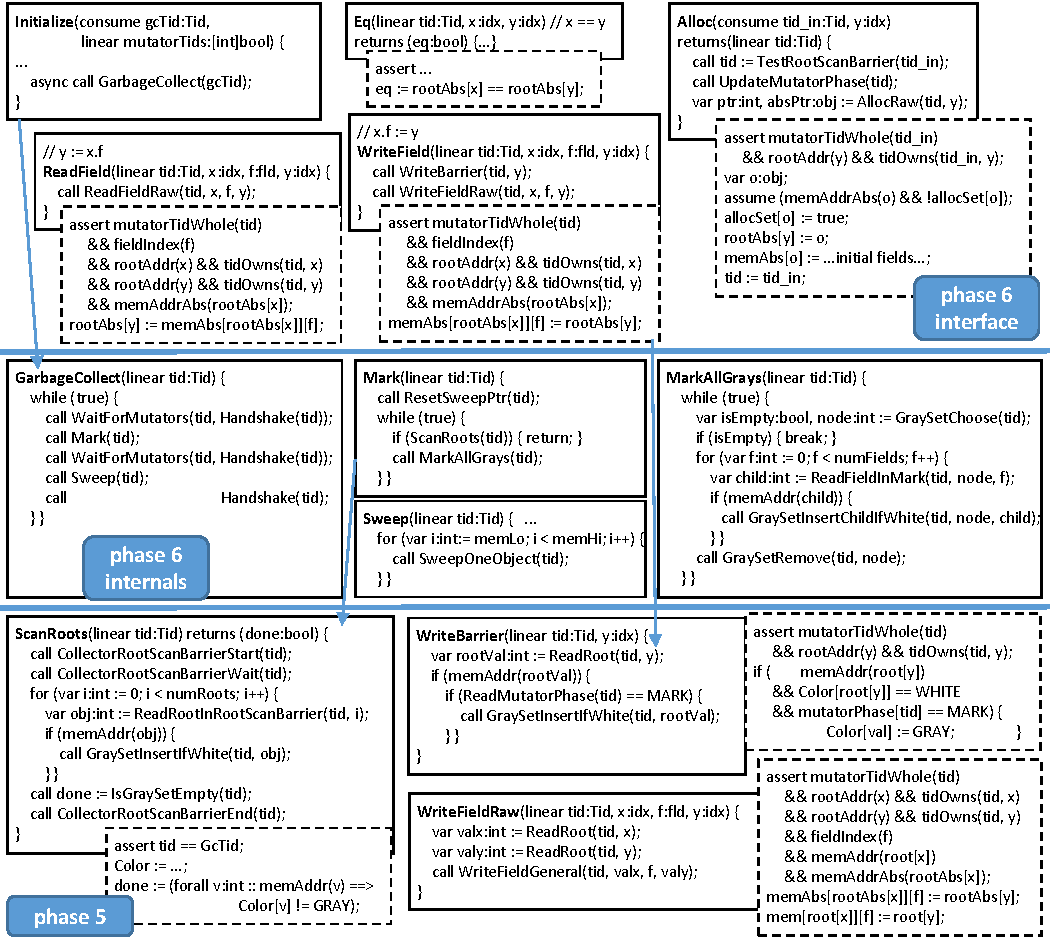
\includegraphics[scale=1.0]{VerifiedGC.pdf}
\caption{Verified garbage collector phases 5, 6 (pseudocode excerpts in solid boxes; atomic action specs in dashed boxes)}
\label{fig:VerifiedGC}
\end{figure*}

We demonstrate the verification methodology and tool on a realistic modern concurrent garbage collector algorithm.
Our algorithm builds on the concurrent collector of Dijkstra et al.~\cite{dijk78}.
Dijkstra's collector is attractive for verification because it maintains a simple tri-color invariant
on the heap objects (in contrast to snapshot-oriented collectors~\cite{doli93,doli94,doma00,azat03}
whose tri-color invariants are more subtle).
By itself, though, Dijkstra's collector is not a modern or performant collector.
First, it becomes incorrect in the presence of more than one program thread (mutator).
Second, it requires that the write-barrier be run not only on updates of heap pointers,
but also on modifications of root pointers, i.e., on modifications of the runtime stacks and the registers;
modern high-performance collectors avoid this overhead.

Therefore, our algorithm (shown inside the solid boxes in Figure~\ref{fig:VerifiedGC}) extends and modifies Dijkstra's collector
to make it work with parallel programs and to not require a write-barrier on root modifications.
Like Dijkstra's collector, our algorithm first {\em marks} all objects reachable from roots (registers and stacks),
shown in Figure~\ref{fig:VerifiedGC}'s Mark procedure, and then {\em sweeps} away all unreached objects,
shown in Figure~\ref{fig:VerifiedGC}'s Sweep procedure.
As in Dijkstra's collector, our algorithm employs a tri-color abstraction to describe the trace of the reachable objects.
Objects are said to be {\em white} if the collector has not seen them yet during the trace.
Objects that the collector encounters become gray and remain gray until the collector scans their children.
Once all the children of an object are noted (meaning that none of them are white), the object becomes black.
The collector works by choosing a node from the set of gray objects (GraySetChoose, called from MarkAllGrays in Figure~\ref{fig:VerifiedGC}),
{\em shading} all its white children to gray (GraySetInsertChildIfWhite), and then removing the object from the gray set by making the object black (GraySetRemove).
The shading operation grays a node if it is white, and does nothing otherwise.
The trace terminates when all roots point to black objects (according to ScanRoots)
and there are no more gray objects (according to IsGraySetEmpty, called by ScanRoots).
Termination is guaranteed because objects can only get darker.
Correctness is guaranteed using an invariant that a black object never points to a white object during the trace
(black objects can only point to gray objects or black objects).
At the end of the trace, objects pointed by the roots must be black, and since no gray objects remain,
black objects only point to black objects,
so the entire set of objects reachable from the roots must be black.

Concurrent mutator operations on objects (ReadField and WriteField in Figure~\ref{fig:VerifiedGC})
could potentially break the no-black-to-white invariant,
because a mutator's WriteField operation could potentially redirect a pointer of a black object to point to a white object.
Therefore, coordination between the program and the concurrent collector is required:
before each raw pointer update (WriteFieldRaw), the WriteField procedure executes a {\em write-barrier} (WriteBarrier).
Before pointer field $x.f$ is set to reference an object $y$,
WriteBarrier shades $y$, ensuring that even if $x$ is black, a pointer from $x$ to $y$
will not violate the no-white-to-black invariant.

The write barrier should shade objects only while the collector is in its mark phase,
not when the collector is sweeping or is idle, and the collector may only switch between phases (mark, sweep, or idle)
when no mutator is in the middle of a WriteField or Alloc operation.
To achieve this (and thereby support correct and efficient support for multiple mutator threads),
we extend Dijkstra's collector with explicit tracking of phases, via a handshaking mechanism~\cite{doli93,doli94}.
A shared variable, collectorPhase, contains the current collector phase.
The collector initiates a handshake by incrementing collectorPhase (in Handshake, called by GarbageCollect).
Each mutator thread keeps cached copy of collectorPhase, and periodically checks to see if
the cached copy mismatches the current collectorPhase, and if so, updates the cached copy
with the most recent value
(in our algorithm, a mutator's call to the allocator, Alloc, checks this in UpdateMutatorPhase,
but the exact location of the check is not critical to correctness).
The GarbageCollector waits until all cached copies equal collectorPhase (WaitForMutators in GarbageCollect),
and then executes a phase (Mark, Sweep, or, for the idle phase, nothing).
Note that each mutator thread can read its own cached phase without acquiring a lock (ReadMutatorPhase in WriteBarrier),
leading to efficient WriteBarrier performance.

Dijkstra's collector requires a write barrier on modifications to roots as well as modifications to objects. 
We eliminate this overhead by employing repeated tracing 
phases until all objects referenced by roots are black. 
A tracing phase starts by stopping all mutators and marking their roots. 
The process of stopping the mutators is similar to a handshake and is done using the CollectorRootScanBarrierStart, CollectorRootScanBarrierWait, and CollectorRootScanBarrierEnd procedures on the collector side and TestRootScanBarrier procedure on the mutator side. 
At the end of the root scan (before the mutators reawaken), all roots point to gray or black objects.
If no gray objects remain (IsGraySetEmpty), then all roots point to black objects, and marking is complete. 
Otherwise, we trace from gray objects until completion and start a new
tracing phase (by stopping the mutators and checking the roots again). 
In a worst-case theoretical scenario we may need to run many root scans and discover more and more white root descendants to trace each time. 
But in practice we usually finish after a small number of scans,
so we obtain correctness and termination in all scenarios and we obtain good performance in real-world scenarios. 

\subsection{Collector Verification in Boogie}
\label{sec:gc-verify}

We have implemented and verified our algorithm in Boogie,
including initialization (Initialize), the GC (GarbageCollect), the allocator (Alloc),
and the mutator operations (ReadField, WriteField, and Eq),
and all the lower-level operations required to implement them (some of these appear
in Figure~\ref{fig:VerifiedGC}; others are omitted from the figure to save space).
To make the verification as realistic as possible,
our Boogie code implements everything in terms of individual CPU operations,
such as load, store, atomic increment/decrement, and CAS (compare-and-swap);
in contrast to some previous work~\cite{gont96},
we do not assume any built-in higher-level operations.
To ease verification, we make some simplifications:
we use a naive allocator (sequential search for free space),
we assume a sequentially consistent memory model,
and we assume that all objects have the same number of fields.
(Except for the assumption of sequential consistency, none of these substantially alter the nature of the proof.)

Overall, our implementation consists of about 2100 lines of Boogie code.
The GC verification takes 60 seconds on the same PC used for microbenchmarks.
The bulk of this time, 54 seconds, is taken by the verification of the refinement checks from Section~\ref{sec:refinement}.
The linear type checking, the yield safety checks, and the commutativity checks take the rest of the time and are insignificant in comparison.

Our verification takes advantage of all techniques in \civl: refinement, assertions, reduction, and linearity.
Refinement gives us extremely simple high-level action specifications for Initialize, ReadField, WriteField, Eq, and Alloc,
shown in their entirety in Figure~\ref{fig:VerifiedGC}'s dashed boxes.
(Initialize and GarbageCollect have empty actions; the GarbageCollector itself is just an internal implementation detail inside Initialize,
which serves only to set up the global GC invariant needed by the other high-level actions.)
Crucially, ReadField, WriteField, Eq, and Alloc appear atomic to mutators, even though internally,
WriteField and Alloc involve many interleaved operations on shared GC data structures.
Figure~\ref{fig:VerifiedGC} shows only shows phases 5 and 6, the two most abstract phases of refinement;
phases 1-4 fill in the implementation details,
such as implementing the set of gray objects as an explicit stack (an array of elements with a pointer to the stack top, in phase 4),
handshaking (phase 3), locks (phase 2), and wrapping the primitive CPU operations in left/right/non-moving atomic actions (phase 1).
Ultimately, the phases are built on trusted CPU-level atomic actions, such as reading and writing roots directly:

\begin{verbatim}
procedure PrimitiveWriteRoot(i:idx, v:int)
  atomic [assert rootAddr(i); root[i] := v;];

procedure PrimitiveReadRoot(i:idx) returns (v:int)
  atomic [assert rootAddr(i); v := root[i];];
\end{verbatim}

We write the highest-level action specifications in terms of an abstract view of memory,
as in earlier work on sequential garbage collector verification~\cite{mccr07,hawb09}.
(Abstract memory is infinite and eternal: once allocated, an abstract object lives forever.
Deallocation is an underlying implementation detail, not exposed in the abstract interface.)
Our abstract view describes a machine as consisting of just three variables:
abstract memory memAbs:[obj][fld]obj, mapping object identifiers and fields to other objects,
abstract root values rootAbs:[idx]obj, mapping root names to objects, and
allocSet:[obj]bool, the set of objects allocated so far.
At this high layer of abstraction, we use Boogie's hiding to hide all other variables
(such as the concrete root set, ``root'', the concrete memory, ``mem'', and the colors, ``Color'', used by lower-level procedures).

All operations are relative to root names of type idx.
ReadField, for example, reads an object field from an object pointed to by root x into a root y.
The predicates rootAddr and tidOwns establish that x and y are valid root names, owned by a particular mutator tid.
(We assume that each root is private to a single mutator stack or register file;
sharing between mutator threads takes place through shared pointers to objects.)
The predicates fieldIndex(f) and memAddrAbs(o) establish that x.f is a valid field of a valid object.
Allocation establishes memAddrAbs(o) for newly allocated objects so that they may be used by subsequent ReadField and WriteField operations.
It also establishes o's unique identity by ensuring that it did not previously belong to the allocated object set.

In addition to atomic action specifications, the verification establishes invariants using assertion reasoning
(omitted from Figure~\ref{fig:VerifiedGC} to save space).
For example, Initialize establishes a global mapping toAbs:[int]obj from physical memory mem and abstract memory memAbs:

\begin{verbatim}
(forall x:int, f:fld ::
   memAddr(x) && toAbs[x] != nil && fieldIndex(f)
  ==> toAbs[mem[x][f]] == memAbs[toAbs[x]][f])
\end{verbatim}

and Mark maintains the no-black-to-white invariant:

\begin{verbatim}
(forall x:int, f:fld ::
  memAddr(x) && Black(Color[x]) && fieldIndex(f)
             && memAddr(mem[x][f]) ==>
  Gray(Color[mem[x][f]]) || Black(Color[mem[x][f]]))
\end{verbatim}

Finally, linearity plays a key role in establishing mutual exclusion.
The GC thread has its own thread id gcTid, and each mutator has its own thread id.
The Initialize procedure consumes gcTid (written here as ``consume'')
and borrows all the mutator thread ids (written as ``linear'', as in Section~\ref{sec:overview}),
so that it's clear that no other concurrent actions are allowed during initialization.
This allows all the internal initialization actions to be both-movers, without requiring any explicit locking.
Initialize must consume gcTid because it passes gcTid to the newly spawned GarbageCollector thread;
since gcTid is consumed, it's impossible to call Initialize twice in an attempt to spawn two parallel GC threads
(which naturally expresses how the algorithm is only safe for a single GC thread).

Because \civl's linearity is based on sets of values,
we can represent thread identifiers as sets that can be subdivided into subsets
(similar to how fractional permissions may be divided into fractions).
During root scanning, each mutator thread places a fraction of its thread id in a global variable,
and reclaims the fraction from the global variable after root scanning completes;
a collector invariant tracks that the global variable contains non-empty fractions from all mutators during root scanning.
Thus, during root scanning, \civl's rules for linearity prove that no interference occurs
between the collector and any mutator operations that require the whole mutator thread id
(``mutatorTidWhole'', used in Figure~\ref{fig:VerifiedGC}'s ReadField, WriteField, Alloc,
and most other mutator operations).

\subsection{Discussion}
We now put atomicity refinement techniques from the literature and
\civl in context by presenting an overview of our design
driver, the stepwise refinement of a garbage collector~\cite{gc-techreport}.
The refinement proof spans six levels of abstraction. 
Each of refinement proof relating two consecutive levels is made feasible by a different
blend of the techniques in \civl. 
% While other refinement techniques have also used garbage collectors as
% case studies, the refinement tasks tackled there bridge only one or two of the levels in 
% our refinement proof\footnote{A more specific discussion of this point
%   can be found in the technical report on the verification of the
%   garbage collector\cite{gc-techreport}.} and only target the refinement verification
% challenges apparent at those levels of the proof. 

The topmost-level description of the garbage collector provides an
idealized, abstract view of memory. 
At this level, none of the lowest-level implementation variables are
visible -- variable hiding has been used to project them away. 
In the top few levels of the garbage collector proof, invariant-based
non-interference reasoning was our primary tool, while reduction
simplified verification by enabling us to use coarser atomic actions and fewer
location invariants.  
Linear variables were used throughout the proof to model the distinct
thread identifiers for the garbage collector thread and mutator
threads, but were most instrumental in encoding single-threaded
execution in the initialization phase of the program. 
For these top few levels of our proof, rely-guarantee and separation-logic-based
approaches would have also performed well, as demonstrated by the
garbage collector proof of Liang et al.~\cite{LiangRGSim}, where
the atomicity of actions in the lower levels our proof is {\em assumed} but not verified.
An important distinguishing capability in \civl is being able to use location invariants rather than pure rely-guarantee reasoning.
This helped interactive proof at the top levels significantly.
For the mark phase of the garbage collector, we made critical use of
different invariants at different locations in procedure bodies. 
While the same non-interference argument could have been encoded in
rely-guarantee reasoning, as we had done ourselves in an earlier
version of our proof, 
it would have required the use of several additional auxiliary shared variables. 
Invariants, rely and guarantee conditions referring to such auxiliary
variables throughout the program made interactive invariant reasoning more difficult to manage. 

In the lower levels of the garbage collector proof, where
correctness of concurrent data structures and synchronization primitives were proven, we made
relatively little use of location invariants, and made heavier use of
linear variables and reduction. 
We also used variable hiding heavily to hide low-level implementation
variables. 
For lower-level refinement tasks, for instance, when verifying the correctness of a
lock-protected concurrently-accessed stack, ownership
arguments, separation logic, or \QED-style atomicity would have been
sufficient. 
But, at the higher levels of our proof, where non-interference
reasoning via invariants and linear variables was indispensable, 
atomicity alone, or ownership or separation logic arguments alone
would have run into difficulty. 

While existing techniques in the literature have as their
``sweet spot'' a few of the refinement proofs in our garbage collector
proof, they run into difficulty in others. 
More critically, they
do not facilitate layering refinement proofs, which is required for stepwise
refinement. 
Using a realistic top-down proof as \civl's design driver led us to
combine in one tool and consistent theory, the verification techniques
of linearity, reduction and non-interference reasoning in the service
of a modular refinement proof directed by the syntactic structure of
the imperative concurrent program. 

%%% SHAZ, I REMOVED THIS SECONDARY NOVELTY POINT, SINCE IT IS MADE
%%% ELSEWHERE IN THE PAPER TOO.
% For this purpose, we also devised
% novel ways to combine automata-theoretic and assertion-based
% verification, and encode the component techniques, e.g., linearity, in
% assertion-based verification.  
% %%%%%%%%% SHAZ PLEASE REFINE OR REMOVE THIS FINAL SENTENCE %%%%%%%%%%%
